\documentclass[12pt]{report}
\usepackage[left=2.5cm,right=2.5cm,top=3cm,bottom=3cm]{geometry}
\usepackage{fancyhdr}
\usepackage{etoolbox}
\usepackage{titlesec}
\usepackage{titling} 
\usepackage{pgfplots}

\pagestyle{fancy}
\fancyhf{} 
\fancyhead[L]{UTN-FRC}
\fancyhead[C]{FISICA ELECTRONICA: TPL1}
\fancyhead[R]{2R3}
\renewcommand{\headrulewidth}{0.4pt}
\fancyfoot[C]{\vfill\thepage}

\patchcmd{\chapter}{\thispagestyle{plain}}{\thispagestyle{fancy}}{}{}

\renewcommand{\chaptername}{Experiencia}

\titleformat{\chapter}[display]
  {\normalfont\huge\bfseries}{\chaptertitlename\ \thechapter}{20pt}{\huge}
\titlespacing*{\chapter}{0pt}{0pt}{0pt}

\DeclareMathSizes{12}{13}{6}{5}

\title{%
  \fontsize{25}{0}\selectfont Universidad Tecnológica Nacional \\
  \fontsize{22}{30}\selectfont Física 2 \\
  \fontsize{18}{25}\selectfont TPL1: Calorimetría
}
\author{
Franco Palombo\\
Gaston Grasso\\
Ignacio Gil\\
Luciano Cortesini\\
}
\date{03 / 10 / 2024}

\begin{document}
%aluminio temp vs tiempo
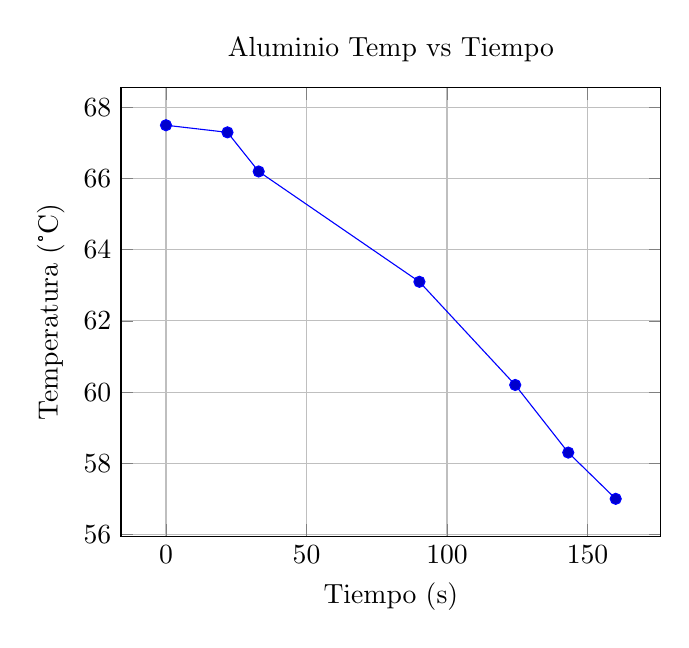
\begin{tikzpicture}
    \begin{axis}[
        xlabel={Tiempo (s)},
        ylabel={Temperatura (°C)},
        title={Aluminio Temp vs Tiempo},
        grid=major,
        legend pos=north west % Posición de la leyenda
    ]
    % Primera función
    \addplot coordinates {
      (0,67.5) (21.87,67.3) (32.98,66.2) (90.17,63.1) (124.26,60.2) (143.13,58.3) (160.01,57)
    };
    \end{axis}
\end{tikzpicture}
%aluminio rad vs tiempo
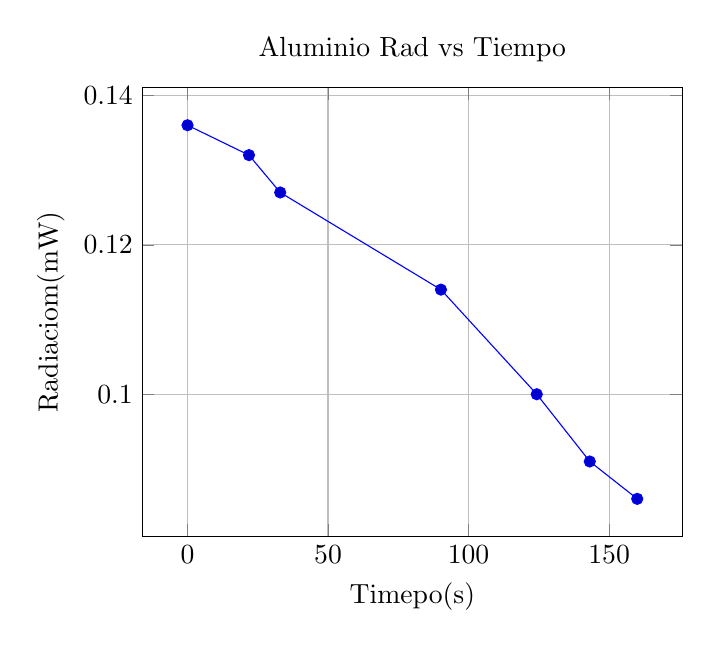
\begin{tikzpicture}
    \begin{axis}[
        xlabel={Timepo(s)},
        ylabel={Radiaciom(mW)},
        title={Aluminio Rad vs Tiempo},
        grid=major,
        legend pos=north west 
    ]
    \addplot coordinates {
    (0,0.136) (21.87,0.132) (32.98,0.127) (90.17,0.114) (124.26,0.1) (143.13,0.091) (160.01,0.086)
    };
    \end{axis}
\end{tikzpicture}\\
%bronce temp vs tiempo
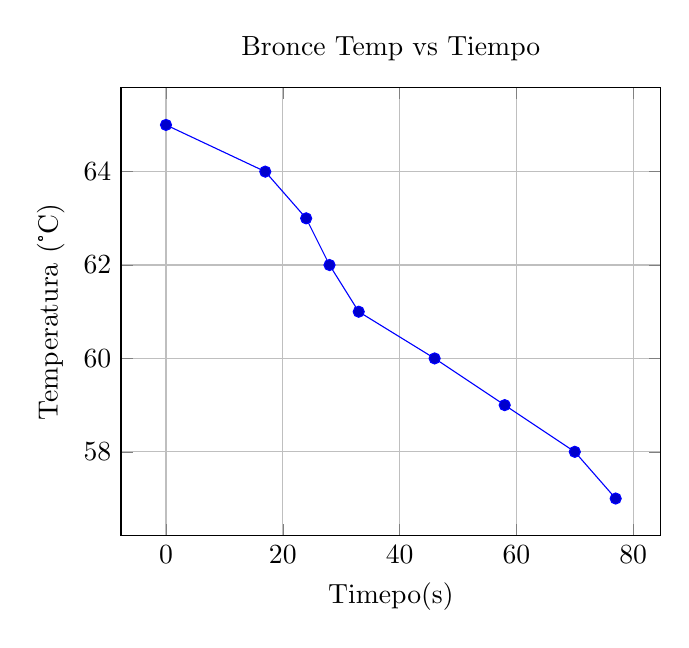
\begin{tikzpicture}
    \begin{axis}[
        xlabel={Timepo(s)},
        ylabel={Temperatura (°C)},
        title={Bronce Temp vs Tiempo},
        grid=major,
        legend pos=north west
    ]
    \addplot coordinates {
      (0,65) (17,64) (24,63) (28,62) (33,61) (46,60) (58,59) (70,58) (77, 57)
    };
    \end{axis}
\end{tikzpicture}
%bronce rad vs tiempo
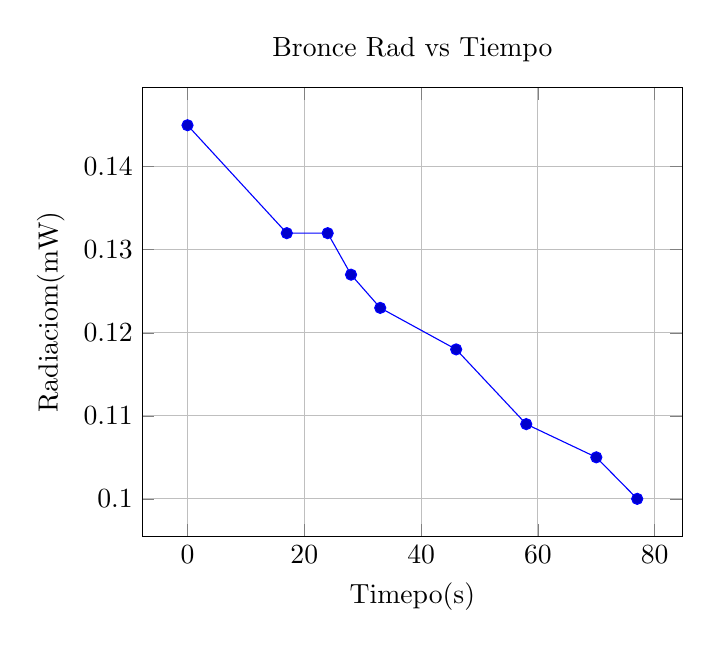
\begin{tikzpicture}
    \begin{axis}[
        xlabel={Timepo(s)},
        ylabel={Radiaciom(mW)},
        title={Bronce Rad vs Tiempo},
        grid=major,
        legend pos=north west
    ]
    \addplot coordinates {
      (0,0.145) (17,0.132) (24,0.132) (28,0.127) (33,0.123) (46,0.118) (58,0.109) (70,0.105) (77, 0.1)
    };
    \end{axis}
\end{tikzpicture}\\


%Plomo Temp vs tiempo
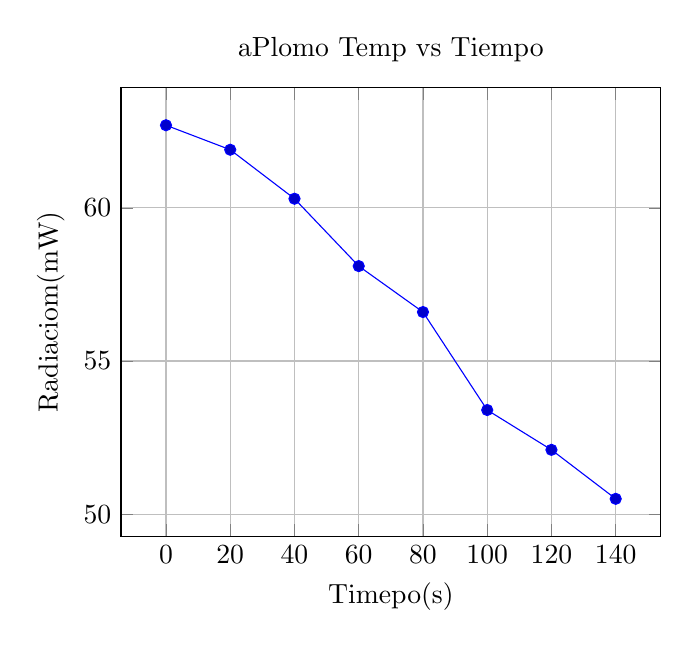
\begin{tikzpicture}
    \begin{axis}[
        xlabel={Timepo(s)},
        ylabel={Radiaciom(mW)},
        title=a{Plomo Temp vs Tiempo},
        grid=major,
        legend pos=north west
    ]
    \addplot coordinates {
      (0,62.7) (20, 61.9) (40, 60.3) (60, 58.1) (80,56.6) (100,53.4) (120,52.1) (140,50.5)
    };
    \end{axis}
\end{tikzpicture}
%Plomo rad vs tiempo
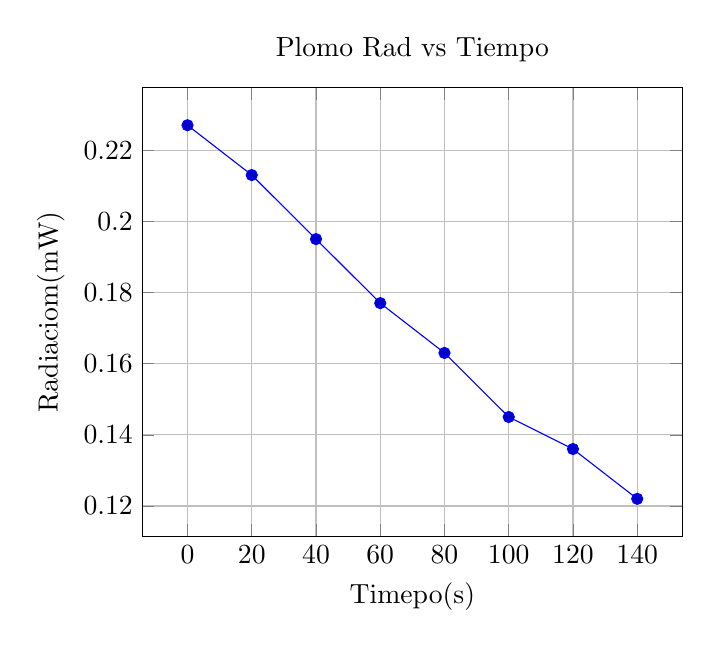
\begin{tikzpicture}
    \begin{axis}[
        xlabel={Timepo(s)},
        ylabel={Radiaciom(mW)},
        title={Plomo Rad vs Tiempo},
        grid=major,
        legend pos=north west
    ]
    \addplot coordinates {
      (0,0.227) (20,0.213 ) (40,0.195) (60,0.177) (80,0.163) (100,0.145) (120,0.136) (140,0.122)
    };
    \end{axis}
\end{tikzpicture}
\end{document}
